\chapter{Labyrinth}

  \section{Motivation}
    Eine einfacher Algorithmus zum Durchfahren eines unverzweigten Labyrinths ist ein Klassiker. Er gehört definitiv zu den Mustdoes zu den Workshops. Jedoch ist es mit den vorhandenen Sensoren schwierig und auch komplex, den Algorithmus so in den Roboter zu programmieren, dass er nicht schnell die Orientierung verliert. Darum müssen, um das Thema schülergerecht anzubieten, einige Vereinfachungen getroffen werden, die auch den Algorithmus vereinfachen. Dazu kann auch noch eine schöne Geschichte gesponnen werden. 

  \section{Geschichte}
    In einer ägyptischen Grabstätte soll der Weg zu einer Grabkammer gefunden werden. Da die Forscher nicht mit dem Fluch des Pharao unliebsame Bekanntschaft machen wollen, soll Eurer Roboter erst einmal vor geschickt werden. Es gilt ein Labyrinth von Gängen zu durchfahren. Als Orientierung stehen lediglich die Wände der Grabkammer zur Verfügung. Glücklicher Weise sind die Wände rechtwinklig angeordnet, sodass es für den Roboter einfacher ist, das Labyrinth zu durchfahren. 

    \begin{capfigure}[Labyrinth]
      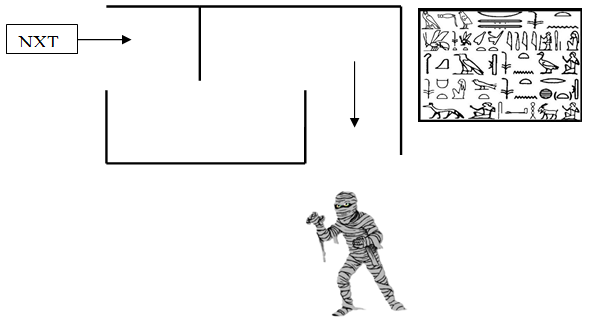
\includegraphics[width=\textwidth]{images/labyrinth}
    \end{capfigure}

  \section{Aufgabenstellung}
    Durchfahrt mit dem Roboter das Labyrinth, ohne die Hieroglyphen an der Wand zu beschädigen (die Wände zu berühren)!
    Es darf nur der Ultraschallsensor verwendet werden.

    Zusatzaufgaben:
    \begin{itemize}
      \item Kehrt um, wenn ihr in einer Sackgasse seid!
      \item Merkt euch den Weg und zeigt diesen auf dem Display an
    \end{itemize}

  \section{Lösung}
    Bei der Lösung fahren wir bis die Distanz zur Wand gering ist. Anschließend dreht sich der Roboter um 90°. Bemerkt der Roboter wieder eine Wand dreht er sich erneut um 180°. Hiernach beginnt das Ganze wieder von Vorne.

    Die Lösung ist auf der DVD unter \textit{Lösungen/Labyrinth} zu finden. Diese umfasst den Programmcode und ein passendes Demovideo
    